\documentclass[10pt,a4paper,notitlepage]{report}
\usepackage[utf8]{inputenc}
\usepackage{amsmath}
\usepackage{amsfonts}
\usepackage{amssymb}
\usepackage{graphicx}
\usepackage{xcolor}
\usepackage{ngerman}
\usepackage[autostyle=true,german=quotes]{csquotes}
\usepackage{picinpar}
\usepackage{geometry}
\geometry{a4paper, top=15mm, left=25mm, right=25mm, bottom=25mm, headsep=10mm, footskip=10mm}
\pagestyle{empty}
\author{Group2}
\renewcommand{\contentsname}{Inhaltsverzeichnis}
\renewcommand{\chaptername}{}
\usepackage{titlesec} 
\titleformat{\chapter}{\bfseries\Huge}{\thechapter.\quad}{0em}{}
\begin{document}

\centering 	{\Huge Konzeptentwurf}\\
		{\large Komplexpraktikum Medieninfromatik - Multimediatechnologie\\}
\
\\
\centering 	07.06.2015\\\
\\
\centering 	Gruppe 2\\
		Gruppenleiter: Alexandra Krien\\
		Bettina Blasberg\\
		Georg Eckert\\
		Stephanie Sara Groß\\
		Philipp Roscher\\\

\tableofcontents
\clearpage\
\\
\begin{flushleft}
\chapter{Einführung}
Wir sind Gruppe 2, die im Rahmen des Komplexpraktikums Medieninformatik, Teilgebiet Multimediatechnologie, eine Spielsoftware entwickelt. 
Unsere Gruppenmitglieder sind dem Titelblatt zu entnehmen.
\section{Aufgabe}
Aufgabe des Komplexpraktikums ist es, in einer Gruppe von fünf Studenten eine Software zu entwickeln.
Spezifisch soll es sich dabei um ein Multiplayer-Spiel handeln, welches das Prinzip der 'Game Orchestration' einbezieht.\\
Bei diesem Konzept handelt es sich um eine Form der Rollenverteilung innerhalb eines Spiels.
Dabei übernimmt einer der Spieler die Rolle des Game Masters der in besonderer Art und Weise Einfluss auf das Spielgeschehen nehmen kann.\\
Dies kann verschiedene Auswirkungen auf die Position des Game Masters gegenüber den weiteren Spielern haben. So kann er sowohl
unterstützend, als auch als Antagonist auftreten.\\
In unserem Spielkonzept entschieden wir uns für die Rolle des Antagonisten.\\
Weitere Vorgaben beschränken sich lediglich auf das Framework libGDX, sowie die Nutzung einer Netzwerkkommunikation. Genauer gehen wir darauf im Bereich 'Technologie' ein.

\chapter{Spielentwurf}
\section{Story}
Im Labyrinth gibt es einen Schatz, der durch einen Drachen beschützt wird. Jedes Kind auf Erden weiß das und träumt davon eines Tages loszuziehen, um den Schatz zu erbeuten. Die Mutigsten reisen von allen Teilen der Welt an, um in das Labyrinth zu treten und Ruhm und Ehre zu erlangen. Dafür müssen sie gegen andere Widersacher antreten und am Ende den Drachen besiegen.\\
\section{Setting}
Es nehmen 5 Spieler teil. Dafür werden zwei Gruppen und ein Game Master durch Zufall entschieden.\\
Der Game Master ist der Drache und muss den Schatz vor den anderen zwei Gruppen beschützen. Dafür hat er verschiedene Fähigkeiten: Er kann die ganze Karte sehen und an den Punkt wo er sich befindet, Schalter betätigen, um Wände zu schieben oder durch geheime Wege zu gehen, die nur er sehen kann. Da er viel strategischer handelt als die anderen Spieler und weniger Lebenspunkte hat, legt er mehr Wert auf seine Verteidigung. Er kann auch Gruppen von Monster hervorrufen und sie zu den anderen Gegner schicken und sie später einsammeln. Aber er kann auch seine Gegner mittels Fallen für kurze Zeit verwirren und sie außer Gefecht setzen.\\
Die zwei Teams bestehen aus jeweils zwei Spielern, einem Kämpfer und einem Heiler. Nachdem diese Aufteilung durch Zufall entschieden wurde, können die Teilnehmer ihre Spielfigur auswählen. Dabei konzentriert sich der Kämpfer eher auf den Angriff und der Heiler auf die Gesundheit seines Teams.\\
Nach der Auswahl fängt das Spiel im Labyrinth an. \\
Dieses wird zufällig generiert und ist somit bei jedem neuen Spielstart anders. Dort befinden sich die Gruppen an verschiedenen Stellen und laufen durch alle Wege, um den Schatz zu bekommen oder gegeneinander zu kämpfen.\\
\section{Rollenverteilung und Charaktere}
Bei den Spielfiguren gibt es eine große Auswahl, denn sie sind nicht nur in Heiler und Kämpfer unterteilt. Sie spezialisieren sich auch durch ihre Kampfposition: Nah-, Mittel- oder Fernkampf.\\
\subsection{Der Drache} 
Der Beschützer des Schatzes und der Herr des Labyrinths. Als Einzelgänger ist er um einiges stärker als ein einzelner Teammitglied. Seine Verteidigung ist entsprechend auch höher als bei den normalen Spieler. \\
\subsection{Fernkampf}
\subsubsection{Schamane}
Ein Magier mit der Fähigkeit, sich von seinem Körper zu trennen und als Geist durch Wände zu gehen. Er kann sich nur bis zu einer gewissen Distanz von seinem Körper entfernen. Dieser kann auch weiterhin angegriffen werden und sollte von seinem Teammitglied verteidigt werden.\\
Schamanen haben außerdem heilende Kräfte.\\
\subsubsection{Bogenschütze}
Seine besondere Attacke sind brennende Pfeile. Wenn er diese schießt, entstehen Flammen auf dem Weg und er blockiert so seinen Gegnern für gewisse Zeit den Pfad.\\
Bogenschützen zählen zu den Kämpfern.\\
\subsection{Mittelfernkampf}
\subsubsection{Ninja}
Neben den Angriffen mit seinen Shuriken und kurzen Schwertern, kann er sich auch für kurze Zeit unsichtbar machen. Dies kostet ihn jedoch viele Angriffspunkte.\\
Ninjas zählen zu den Kämpfern.\\
\subsubsection{Hexe}
Eine Magierin, die mit ihren besonderer Tränke kämpft. Gegen ihre Gegner wirft sie Gifttränke, um sie zu schwächen und für sich oder ihren Partner benutzt sie Heiltränke. Ist die Situation besonders heikel, kann sie auf ihrem Besen reiten und schnell von einem Ort fliehen.\\
\subsection{Nahkampf}
\subsubsection{Schwertkämpfer}
Er kann mehrere Male hintereinander mit seinem Schwert angreifen und sich mit dem Schild verteidigen. Die besondere Fähigkeit ist der Kampfschrei, womit er seine Gegner für kurze Zeit verwirren und aufhalten kann.\\
\subsubsection{Kämpfer}
Seine einzigen Waffen sind seine Hände und somit ist er für den Nahkampf besonders gut geeignet. Er hat die Fähigkeit mit einem besonders festem Schlag seine Gegner für kurze Zeit K.O. zu schlagen.\\
Außerdem trägt er immer Verbandszeug mit sich und zählt dadurch zu den Heilern.\\
\section{Ziel}
Um den Schatz zu erbeuten benötigt man den Schlüssel der Schatzkammer. Dieser ist in 3 Teile zerbrochen und jede Partei, also jedes Team und auch der Drache, besitzen zu Anfang genau einen davon. Wird ein Team besiegt, so erhält jenes Team bzw. der Drache, welches den entscheidenden Angriff geführt hat das Schlüsselfragment. Die besiegte Partei darf nach einer kurzen Auszeit am ursprünglichen Startpunkt von vorn beginnen und erhält somit die Gelegenheit Schlüsselteile zurück zu erobern. Erlangt ein Team oder der Drache alle 3 Teile und schafft es ohne zu sterben zum Schatz, so ist das Spiel gewonnen.\\

\chapter{Design}
Das Spiel wird ein Top-Down-Spiel in 2-D. Entsprechend wird das gesamte Design im Pixelstil gehalten.\\
Zur Charakterauswahl werden etwas größere und detailreichere Bilder angezeigt und im Spiel selbst typische Retro-Pixelgrafik verwendet.\\
Es soll keine Unterschiede in der Grafik zwischen PC und Android geben.\\
Die folgenden Grafiken sind erste konzeptuelle Entwürfe und dienen lediglich einer ersten Veranschaulichung.\\

\section{Welt}
	\begin{center}
			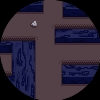
\includegraphics[scale=3]{Maze.jpg}\\
		Die Spieleransicht\\
	\end{center}

\section{Spielfiguren}
\begin{center}
	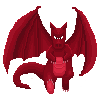
\includegraphics[scale=3]{Dragon.png}\\
	Der Drache\\
		
	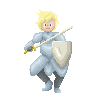
\includegraphics[scale=2]{Knight.png}
	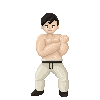
\includegraphics[scale=2]{Fighter.png}\\
	Der Schwertkämpfer und der Faustkämpfer\\
	
	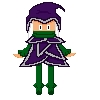
\includegraphics[scale=2]{Witch}
	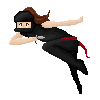
\includegraphics[scale=2]{Ninja}\\
	Die Hexe und der Ninja\\
	
	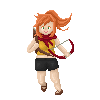
\includegraphics[scale=2]{Archer}
	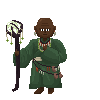
\includegraphics[scale=2]{Shaman}\\
	Der Bogenschütze und der Schamane\\

	\end{center}
\chapter{Technologie und Steuerung}
Das Spiel wird sowohl auf PC als auch auf Android Endgeräten spielbar sein.\\
Die Unterschiede werden möglichst gering und auf die Steuerung und für den Spielablauf unbedeutende Elemente, wie bestimmte Effekte, beschränkt sein. So wird die Figur auf dem Smartphone mit dem Finger bewegt und auf dem PC der Finger durch die Maus ersetzt.\\
Voraussetzung für das Spiel ist ein Endgerät mit respektive Windows 7 oder höher, Linux mit Kernel 3.16 oder höher, Android 4 oder höher. Wir behalten uns vor Android als einzige Zielplattform zu setzen, falls Smartphone-Sensoren in das Bedienkonzept einfließen sollten. Das Gerät muss Open GL unterstützen und netzwerkfähig sein. Oracle Java muss mindestens in Version 1.6 installiert sein. Für ein gutes Spielerlebnis werden mindestens Geräte mit 2 Prozessorkernen > 1GHz und einer Bildschirmauflösung von 480x800 Bildpunkten empfohlen.

\chapter{Planung}
\section{Aufgabenverteilung}
Für den Prototypen soll Georg sich um den Start des Projektes in einer leeren Welt kümmern und die Spielfigur mit der Bewegungsfunktion ausstatten (5.1.1.1). Alexandra übernimmt die Erstellung einer simplen Welt (5.1.1.2.). Sara, Nathalie und Philipp kümmern sich um die verschiedenen Spielklassen (5.1.1.3.).\\
Für die späteren Aufgaben gibt es noch keine Zuweisung. Geplant ist jedoch, für jedes Aufgabengebiet einen Hauptverantwortlichen festzulegen, der darüber einerseits besonders gut Bescheid weiß, Schnittstellen zu anderen Programmteilen festlegen und anderen helfen kann, andererseits aber auch einen Überblick über das Aufgabenfeld haben sollte und der durch Verteilung von spezifischen Aufgaben eine rechtzeitige Fertigstellung der jeweiligen Arbeitspakete garantieren soll.\\
\subsection{Prototyp}

\subsubsection{Charakterbewegung}
Im Prototyp sollen die elementaren Bewegungsfunktionen des Charakters enthalten sein. Die Steuerung auf Android-Geräten wird durch Berührung des Touchscreens realisiert und soll intuitiv sowie verzögerungsfrei funktionieren. Durch entsprechende Sprites wird die aktuelle Bewegungsrichtung dargestellt. Zudem bewegt sich der Charakter schneller, je weiter der Finger von ihm entfernt ist, überschreitet jedoch eine gewisse Höchstgeschwindigkeit nicht.

\subsubsection{Welt}
Der Prototyp sollte zum Test der Bewegungsfunktionen eine vorgefertigte Spielwelt enthalten, die noch keinerlei zufälliger Erstellung bedarf.

\subsubsection{Spielcharaktere (Game Master, Klassen)}
Der Prototyp soll eine grundlegende Charakterauswahl bieten, in dem man zwischen einigen verschiedenen Charakterklassen wählen kann. Im Spiel soll dies sich zumindest durch eine entsprechende Anpassung des Sprites bemerkbar machen.

\subsection{Gestaltung}
Alle nötigen Sprites müssen entweder erstellt oder unter Beachtung entsprechender Lizenzen übernommen werden. Dazu zählen beispielsweise: Spielcharaktere (Game Master, Klassen), Welt (Boden, Wände), Items.

\subsection{Programmierung}

\subsubsection{Levelgenerierung + Karte}
Das Spiel soll zufällig erstellte Welten beinhalten. Dafür ist ein entsprechender Algorithmus zu integrieren, der auch garantiert, dass das Level abgeschlossen werden kann und kein Spieler \enquote{gefangen} sein kann. An dieser Stelle ist zu beachten, dass – um das Spiel nicht zu unfair und unspaßig zu gestalten – auf das Balancing geachtet wird, also dass nicht ein Team durch die Positionierung von Spawnpoints/Items/etc. einen erheblichen Vorteil gegenüber einem anderen hat. An die Levelerstellung ist die Karte gebunden, die von den Spielern aufgerufen werden kann, um die bisher schon erforschten Gebiete darzustellen. Die Levelgenerierung kann sich dabei auf ein Arrangement bereits vorgefertigter Labyrinthteile beschränken.

\subsubsection{Bewegung}
Die Steuerung sollte natürlich weiterhin den Anforderungen, die schon im Prototyp verlangt waren, genügen. An dieser Stelle ist allerdings eventuell hinsichtlich der Netzwerkübertragung noch etwas Optimierung nötig. 

\subsubsection{Kampf} 
Einen essentiellen Part des Spiels nehmen die Kämpfe ein. Hier ist beispielsweise die Implementierung der speziellen Fähigkeiten der verschiedenen Charakterklassen nötig. Ein entsprechendes Lebens-/Schadenssystem ist notwendig, um Kämpfe fair zu gestalten. Um alle Klassen am Ende mehr oder weniger gleich stark machen zu können, ist eine Umsetzung mit vielen Variablen (Leben, Angriffsschaden, …) zum Finetuning dieser Werte wünschenswert. 

\subsection{Netzwerkkommunikation (Schnittstelle)}
Einen sehr wichtigen Bestandteil des Spiels stellt das Networking da. Um eine gute User Experience zu schaffen, muss das Spiel schnell auf Geschehnisse (Bewegung, Kämpfe) reagieren. Unter Beachtung der Latenz und Zuverlässigkeit des verwendeten Netzwerks muss eine regelmäßige Synchronisation des Spielzustands stattfinden, um alle Spieler auf den aktuellen Stand zu bringen. Gut geeignet ist vermutlich eine Server-Client-Architektur, um die Spielberechnung zu zentralisieren und die Android-Geräte etwas zu entlasten. 

\subsection{Charakterlogik} 
Neben den bereits erwähnten individuellen Angriffen und Fähigkeiten werden natürlich noch andere Funktionen für die Spieler benötigt, wie z.B. ein Respawn nach Verlust aller Lebenspunkte. Weiterhin müssen die speziellen Fähigkeiten des Game Masters implementiert werden.

\subsection{Gegenstände}
Gegenstände sollen Spieler oder Teams in gewissen Aspekten verstärken. Dafür ist eine Implementierung der jeweiligen Funktionalitäten notwendig. Um die Items mitnehmen zu können, werden die Spieler Maps haben, wo der Schlüssel das gefundene Objekt und der Wert die Anzahl davon ist.

\subsection{Menü}
Eine simple Hauptmenüführung soll auch Spielern ohne technische Kenntnisse ermöglichen, ohne weiteres einem Spiel beitreten zu können. Es sollte nicht zu überladen und vom grafischen Stil an das Game Art angelehnt sein. Im Spiel sollte das User Interface einen möglichst geringen Anteil des Spielfensters einnehmen, um die Sicht auf das Spiel nicht zu versperren, jedoch trotzdem noch einfach bedienbar bleiben. 

\subsection{Ton} 
Eine Aufgabe für den späteren Projektverlauf ist die Unterlegung des Spiels mit Musik. An dieser Stelle kann unterschieden werden zwischen statischer Hintergrundmusik sowie Sounds, die sich am Gameplay orientieren, also beispielsweise an der Bewegung und den Kämpfen.

\section{Arbeitsplan}
Ein Arbeitsplan wurde zum jetzigen Zeitpunkt noch nicht erarbeitet.

\chapter{Ergänzungen}
In Folge der ersten Konzeptpräsentation haben wir weitere Planung vorgenommen und folgende Punkte festgelegt:\\
Die Kamera soll vorerst zentral auf dem Spieler fixiert sein. Eventuell ändern wir das im Verlauf der Entwicklung ab, so dass die Kamera mitscrollt wenn man \enquote{gegen den Rand} läuft, mit mehr Sicht in die Richtung, in die man läuft.\\
Wir wollen mit Box2D als Collider/ zur Collision Detection arbeiten.\\
Beim spawnen von Gegenständen (z.B. Pfeile beim Bogenschießen) soll mit Pools gearbeitet werden, damit Objecte recyclt werden können.\\
Klickt der Spieler auf die Karte, läuft der Charakter dorthin. Klickt man auf einen Gegner, wird ein Angriff ausgeführt. Ist man dabei außer Reichweite läuft der Charakter automatisch näher heran und greift daraufhin an. Sollte der Gegner sich ebenfalls bewegt haben und so nicht nah genug sein wird kein Angriff ausgeführt und der Spieler muss weiter auf den Gegner klicken.\\
Jedes Team hat einen Rückzugsraum. Dieser ist der Ort, wo sie ihr Spiel angefangen haben. Sollte ein Mitglied besiegt werden, wird er wiederbelebt und an dem Punkt geschickt. Dort hat er für eine begrenzte Zeit Schutz. Dieser Ort ist auch nur für das eigene Team erreichbar.\\
Im Labyrinth kann man an verschiedenen Stellen Schatztruhen finden. Diese werden von Anfang als Teil der Karte generiert. Sie sind an den gleichen Stellen, dennoch haben sie bei jedem neuen Spiel einen anderen Schatz. Man hat von diesen eine Große Auswahl, jedoch werden nur 70 Prozent der vorgefertigten Sprites verwendet.\\


	\begin{center}
		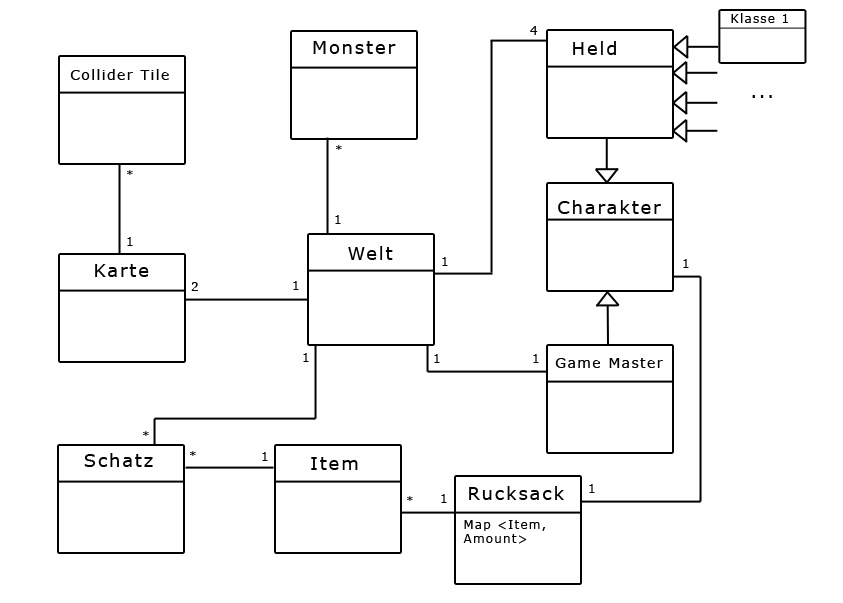
\includegraphics[scale=0.5]{Class-Diagram.jpg}\\
		Ein grobes Klassendiagramm, dass wir zusammengestellt haben.
		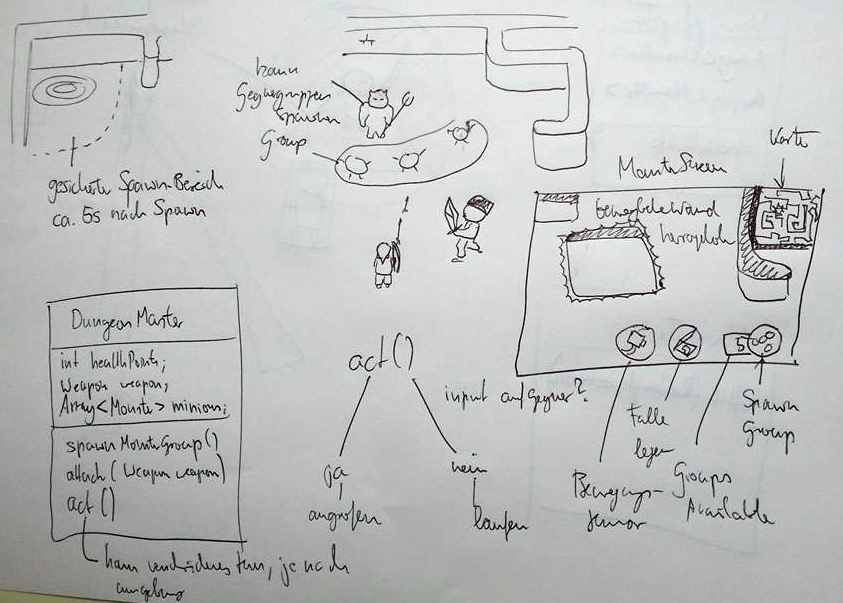
\includegraphics[scale=0.5]{scetch_01.jpg}
		Notizen zum Kampfsystem und Steuerung für den Game Master.
	\end{center}
	
\end{flushleft}
\end{document}
